\documentclass{mlnotes}
\usepackage{graphicx}
\graphicspath{ {./images/ } }

\lecture{7}
\topic{Decision Trees}
\author{Aru Gyani}
\subtitle{Based on Prof.\ Rishabh Iyer's slides.}

% --- Links --- %
\def\seeingtheory{https://seeing-theory.brown.edu/basic-probability/index.html}
\def\khanstats{https://www.khanacademy.org/math/ap-statistics/probability-ap/stats-conditional-probability/a/check-independence-conditional-probability}
\def\byjus{https://byjus.com/maths/intersection-of-sets/}
\def\thoughtco{https://www.thoughtco.com/multiplication-rule-for-independent-events-3126602}

\begin{document}
\maketitle
\tableofcontents
\clearpage

\part{Probability, Random Variables, and Entropy}
\section{Probability}
The following content is sourced from the following:
\begin{itemize}
  \item \link{\seeingtheory}{seeing-theory}
  \item \link{\khanstats}{Khan Academy}
  \item Professor Rishabh Iyer's class notes
  \item \link{\byjus}{BYJU'S}
  \item \link{\thoughtco}{ThoughtCo}
\end{itemize}

\subsection{Discrete Probability}

\begin{definition}{Sample space}{sample_space}
  \define{Sample space} specifies the set of possible outcomes.\\[12pt]
  For example, \(\Omega=\{H,T\}\) would be the set of possible outcomes of a
  coin flip. Simply put, we are saying a coin flip could be either
  \emph{heads} or \emph{tails}.
\end{definition}

\begin{definition}{Probability}{probability}
  \define{Probability} is simply how likely something is to happen\\[12pt]
  For each element \(\omega\) inside of our sample space \(\Omega\), there is a
  number \(p(\omega)\ \epsilon\ [0,1]\) called a probability. This represents
  how likely the event \(\omega\) is to happen.\\[12pt]
  The total probability of all possible outcomes (each outcome being an element
  \(\omega\)) within the sample space \(\Omega\) adds up to \(1\). This means
  that one of the outcomes in the sample space is certain to occur.
  
  \[
    \sum_{\omega \in \Omega} p(\omega) = 1
  \]

  For exaxmple, a biased coin might have \(p(H) = .6\) and \(p(T) = .4\).
  \\[12pt]
  \small{Note: \([0,1]\)} is a range, not a set. This number is always between 0
  and 1, where 0 indicates impossibility and 1 indicates certainty.
\end{definition}

\begin{definition}{Event}{event}
  An \define{event} is a subset of the sample space \(\Omega\), e.g.
  \begin{itemize}
    \item Let \(\Omega = \{1,2,3,4,5,6\}\) be the \(6\) possible outcomes of a
    dice roll.
    \item \(A = \{1,5,6\} \subseteq \Omega\) would be the event that the dice roll
    comes up as a one, five, or six.
  \end{itemize}

  The probability of an event is just the \underline{sum of all the outcomes
  that it contains}.
  \[
    p(A) = p(1) + p(5) + p(6)
  \]
  \small{Note: \(A \subseteq\ \Omega\) means that \(A\) is a subset of \(\Omega\). Below, is a brief recap of what a subset is.}
  \begin{definition}{Subset}{subset}
    A set \(A\) is a\ \define{subset} of another set \(B\) if all of
    elements of the set \(A\) are elements of the set \(B\). In other words, the
    set \(A\) is contained inside the set \(B\).
  \end{definition} 
\end{definition}

\subsection{Conditional Probability}
\subsubsection{Independence}
We say two events are independent if knowing one event occurred doesn't change
the probability of the other event.
For example, the probability that a fair coin shows ``heads'' after being
flipped is \(\frac{1}{2}\). What if we knew the day was Tuesday? Does this
change the probability of getting ``heads''? Of course not. The probability of
getting ``heads'', given that it's a Tuesday, is still \(\frac{1}{2}\). Thus,
the result of a coin flip and the day being Tuesday are independent events.
\link[blue]{\khanstats}{More reading}.

\begin{definition}{\define{Independence}}{independence}
  Two events \(A\) and \(B\) are independent if
  \[
    p(A \cap B) = p(A)p(B) 
  \]

  Informally, \(p(A \cap B)\) indicates the probability of \(A\) and \(B\) (aka
  probability of \(A\) intersection \(B\)). This means that it indicates the
  likelihood of both events happening.
  \\[12pt]
  Now, when we multiply \(p(A)p(B)\), we are calculating the probability that
  \(A\) occurs and then, independently, that \(B\) occurs. 
  \\[12pt]
  The probability that both events occur simultaneously (the intersection) is
  the product of their individual probabilities.

  \begin{definition}{\define{Multiplication Rule}}{multiplication_rule}
    The \textbf{multiplication rule} for independent events relates the
    probabilities of two events to the probability that they both occur. 
    \\[12pt]
    For example, suppose that we roll a six-sided die and then flip a coin.
    These two events are independent. The probability of rolling a \(1\) is
    \(\frac{1}{6}\). The probability of a head is \(\frac{1}{2}\). The
    probability of rolling a \(1\) \emph{and} getting a head is \(\frac{1}{6} * \frac{1}{2} = \frac{1}{12}\)
  \end{definition}
  
  \begin{definition}{\define{Intersection}}{intersection}
    The intersection of sets \(A\) and \(B\) is the set of all elements which
    are common to both \(A\) and \(B\).
    \\[12pt]
    Suppose \(A\) is the set of even numbers less than \(10\) and \(B\) is the
    set of the first five multiples of 4, then the intersection of these two can
    be identified as:
    \begin{align}
      A = \{2,4,6,8\}\\
      B = \{4,8,12,16,20\}
    \end{align}
    The elements common to \(A\) and \(B\) are \(4\) and \(8\). Therefore, the
    set of elements in the intersection A and B is:
    \[
      P(A \cap B) = \{4,8\}
    \]
  \end{definition}
\end{definition}
\vspace{12pt}
\paragraph{Independence Example 1}
Let's suppose that we have a fair die: \(p(1) = \cdots = p(6) = \frac{1}{6}\) (the
probability of rolling any number on the dice is equal). If \(A = \{1,2,5\}\)
and \(B = \{3,4,6\}\) are \(A\) and \(B\) independent?

No, they aren't independent. We know this because the intersection of \(A\) and
\(B\) is \(P(A \cap B) = \{\} \text{ or } \emptyset \). This means that their
intersection has a probability of \(0\), meaning it will never happen. Compare this to
\(P(A)P(B)\) and we find that:
\begin{gather*}
P(A) = P(1) + P(2) + P(5) = \frac{3}{6}\\
P(B) = P(3) + P(4) + P(6) = \frac{3}{6}\\
P(A)P(B) = \frac{3}{6} * \frac{3}{6} = \frac{1}{4} = 0.25
\end{gather*}

Thus, given that \(P(A)P(B)\) represents the probability of both \(A\) and \(B\)
occurring independently (see Definition 1.6: Multiplication Rule), we find that
the intersection does not equal their independent occurrence. This means that
\(A\) and \(B\) are \underline{not independent}.

\paragraph{Independence Example 2} Now, suppose that \(\Omega =
\{(1,1),(1,2),\cdot,(6,6)\}\) is the set of all possible rolls of two
\textbf{unbiased} dice.
\begin{itemize}
  \item Let \(A = \{(1,1),(1,2),(1,3),\cdot,(1,6)\}\) be the event that the
  first die rolls a \(1\).
  \item Let \(B = \{(1,6),(2,6),\cdot,(6,6)\}\) be the event that the second die
  rolls a \(6\).
\end{itemize}

Are \(A\) and \(B\) independent?
\begin{figure}[ht]
  \centering
  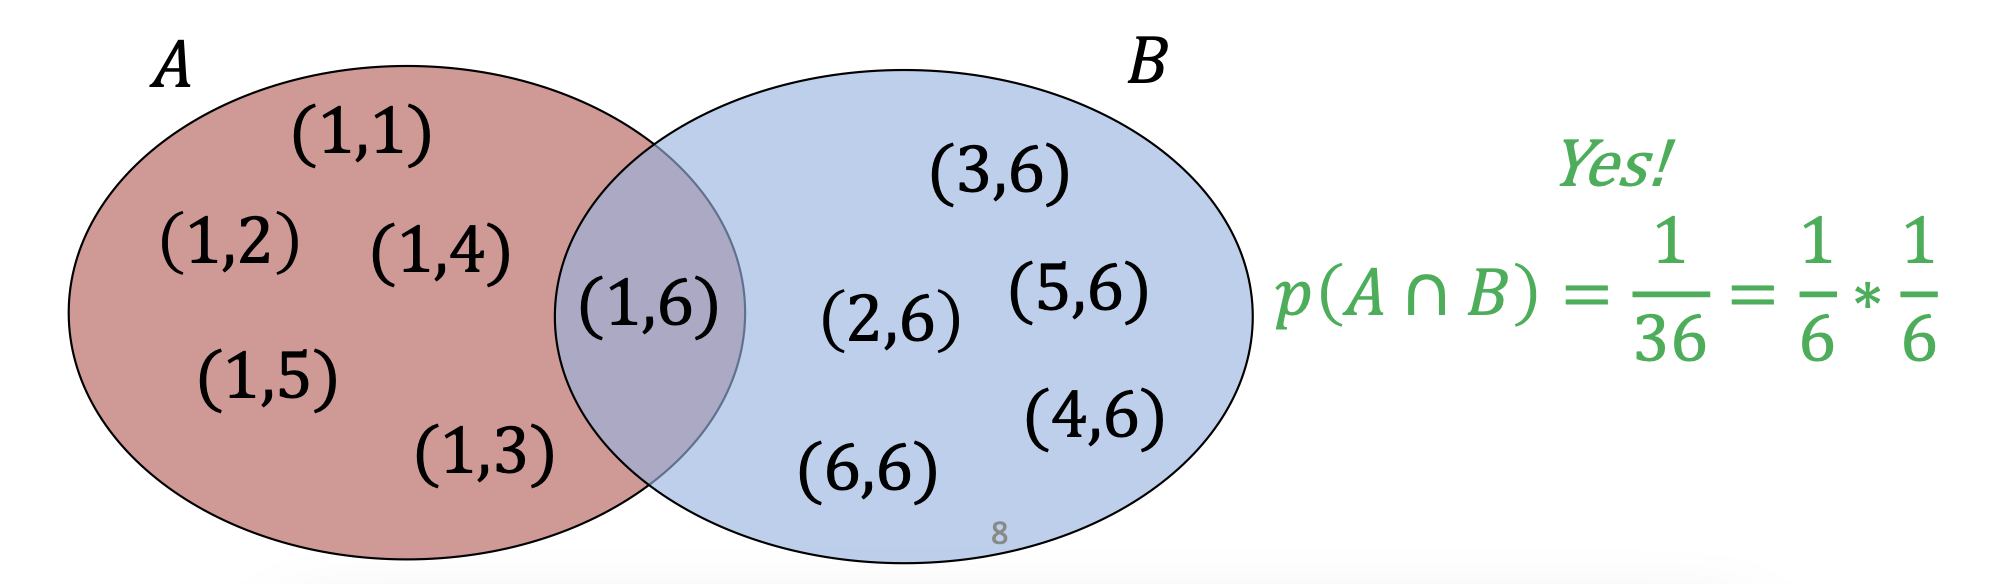
\includegraphics[width=15cm]{images/image.png}
\end{figure}

\subsubsection{Conditional Probability}
\begin{definition}{\define{Conditional Probability}}{conditional_probability}
  The \textbf{conditional probability} of an event \(A\) given an event \(B\)
  with \(B\) with \(p(B) > 0\) is defined to be:
  \begin{align*}
    p(A|B) &= \frac{p(A \cap B)}{p(B)}
  \end{align*}
  This formula tells us that to find the probability of \(A\) given \(B\), you
  divide the probability of both \(A\) and \(B\) occurring together by the
  probability of \(B\) occurring.
  \\[12pt]
  Note: The vertical bar ``|'' means ``given''. So, \(P(A | B)\) can be read as
  ``the probability that Event \(A\) occurs \underline{given} Event \(B\) has
  occurred''.
  \\[12pt]
  This is the probability of the event \(A \cap B\) happening over the sample
  space \(\Omega' = B\).
  \\[12pt]
  Properties of Conditional Probability:
  \begin{itemize}
    \item \(\sum_{\omega \in \Omega'} p(\omega|B) = 1\)
    \item If \(A\) and \(B\) are independent, then \(p(A|B) = p(A)\).
    \begin{align*}
      p(A|B) &= \frac{p(A \cap B)}{p(B)}\\
             &= \frac{p(A)p(B)}{p(B)}\\
             &= p(A)
    \end{align*}
  \end{itemize}
\end{definition}

\paragraph{Conditional Probability Example 1: Dice Rolls}
To demonstrate the calculations of conditional probability, let's take two
events.
\begin{itemize}
  \item \(A = \{\text{Dice Roll is even}\} = \{2,4,6\}\)
  \item \(B = \{\text{Dice Roll > 4}\} = \{5,6\}\)
\end{itemize}

Conditional probability is about looking at what the chances are of one thing
happening if we know that something else already happened.
\\[12pt]
\(P(A|B)\): ``If we know that the dice is greater than \(4\), what's the chance
it's also even?''

To figure this out let's go through the following steps:
\begin{enumerate}
  \item Look at the potential outcomes in \(B\), which are \(\{5, 6\}\).
  \item From those, find the ones that are also in \(A\). Only the number \(6\)
  is both greater than 4 and even.
  \item Since there are two numbers in \(B\) and only one of them is also in
  \(A\), the conditional probability \(P(A|B)\) is \(\frac{1}{2}\).
\end{enumerate}

Since we know \(B\) has happened, we know we are only looking at a world where
the dice roll is \(5\) or \(6\) (\(> 4\)). In that world, there's only one even
number, which is 6.\ \textbf{Conditional probability adjusts your focus}.
Instead of looking at all possible dice rolls, you're only looking at the ones
where \(B\) is true. Then you check, out of those, how often \(A\) is true.
\\[12pt]
\textbf{\underline{Question}}: How is the probability \(\frac{1}{2}\) when we aren't
guaranteed a \(6\) when we look \(A\) (it could also be \(5\)).
\\[12pt]
When we calculate the conditional probability \(P(A|B)\), we are not talking
about rolling the dice again. We're talking about a scenario where we already
know that a certain event (in this case, event \(B\): rolling a number greater
than \(4\)) has occurred. This knowledge ``shrinks'' our sample space --- the
set of possible outcomes we consider --- to only those that fit this condition.
\\[12pt]
So, when we're looking at \(P(A|B)\), we're asking ``Given that we have rolled a
number greater than 4, what is the probability that this number is also even?''
\\[12pt]
Since we know that \(B\) has happened, we ignore the rest of our original sample
space of the dice \((1,2,3,4)\) and only consider \(\{5,6\}\). Out of these two
possible outcomes, what's the probability the number we rolled is even? Thus, we
reach at \(\frac{1}{2}\).
\\[12pt]
To show this same process done using the formula\ldots
\begin{align*}
  p(A|B) &= \frac{p(A \cap B)}{p(B)}\\
  p(A \cap B) &= p(6) = \frac{1}{6}\\
  p(B) &= p(5) + p(6) = \frac{1}{6} + \frac{1}{6} = \frac{1}{3}\\
  \frac{p(A \cap B)}{p(B)} &= \frac{\frac{1}{6}}{\frac{1}{3}}\\
                           &= \frac{1}{6} * \frac{3}{1}\\ 
                           &= \frac{1}{2}
\end{align*}

\section{Discrete Random Variables}
\section{Entropy}
\subsection{Conditional Entropy}
\subsection{Information Gain}

\part{Decision Trees}

\phantomsection{}
\addcontentsline{toc}{part}{Index}
\printindex[defn]
\end{document}